\chapter{基于内容的推荐系统:最新技术和趋势}

\section{简介}
网络和数字图书馆中蕴含着丰富的信息,它们往往是动态而且异构,这决定了我们很难迅速找到我们的需求。

因此,用户建模和个性化信息的获取变得非常重要:用户根据他们的兴趣和品位,需要大量的可用的信息来支持他们的个性化选择。

许多用户的个性化信息内容被加入到推荐系统中[73]。推荐系统引导用户对大量感兴趣和有用的东西进行个性化选择[17]。推荐系统算法使用关于消费者兴趣的输入产生一个推荐列表。在Amazon.com,推荐系统算法被用于为每个消费者提供在线的个性化服务,例如,给软件工程师展示编程类的商品,为新妈妈展示宝宝的玩具[50]。

推荐系统的问题已经被广泛研究,而且出现了两个范式。基于内容的推荐系统尝试尝试推荐那些用户过去喜欢的产品的相似产品,而协同推荐范式识别那些偏好相似的用户,推荐他们喜欢的产品[7]。

本章中,将对基于内容的推荐系统进行全面系统的研究,分为两个部分:
\begin{itemize}
	\item 提供最新技术的一个大纲,包含那些最有效的应用最广泛的技术。
	\item 阐述基于内容的推荐系统未来发展的趋势和方向。
\end{itemize}

\section{基于内容的推荐系统基础}
基于内容的推荐方法分析用户曾经评分过的产品的描述性文档,然后基于产品为用户兴趣建模[63]。推荐过程基本上是匹配用户侧写的属性和内容目标的属性。

\subsection{基于内容系统的体系结构}
基于内容的推荐系统的体系结构如图1.1所示
\begin{figure}[!htb]
	\centering
	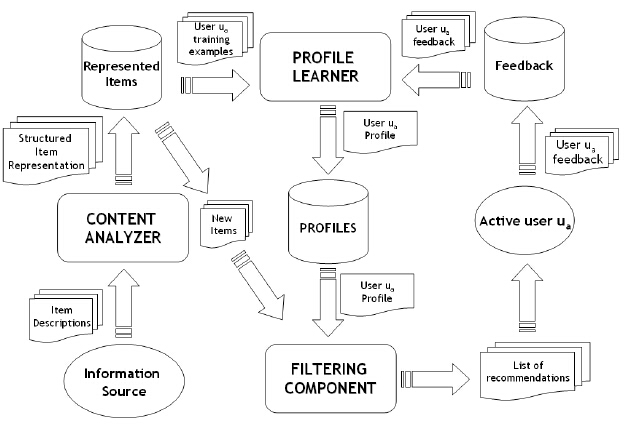
\includegraphics[scale=0.5]{figure/f3.1.jpg}
	\caption{基于内容的推荐系统的体系结构}
\end{figure}

如上图所示,生成推荐的过程主要依靠三个部件:
\begin{itemize}
	\item 内容分析器:从原先的商品信息(例如文档、网页、新闻、产品描述)中提取有用的信息用一种适当的方式表示。例如(将网页表示成关键词向量)该表示形式将作为属性学习器和过滤部件的输入结点。
	\item 文件学习器:该模块收集、泛化代表用户偏好的数据,生成用户概要信息。通常,是采用机器学习方法从用户之前喜欢和不喜欢的商品信息中推出一个表示用户喜好的模型。例如,一个基于网页的推荐系统的属性学习器能够实现一个相关反馈的方法,将表示正面和负面例子的向量与表示用户概要信息的原型向量混合在一起。训练样例是那些附有用户正面和负面反馈信息的网页。
	\item  过滤部件:通过学习用户概要信息,匹配用户概要信息和商品信息,推荐相关的商品,结果是一个二元的连续型的相关判断(相似度度量)。后者将生成一个用户可能感兴趣的潜在商品评分列表。该匹配是计算原型向量和商品向量的余弦相似度。
\end{itemize} 

推荐过程的第一步是内容分析器所表现的,通常用到的技术来自信息检索系统[80,6]。来自信息源的项目描述通过内容分析器处理,提取特征(关键词、n-grams,概念,\dots)。

为了使目标用户$ u_a $的属性能够结构化和能更新,ta对产品的反映会在某个方式下被记录。这些反映,被称为注解或反馈[39],它们伴着产品描述一起出现。

记录用户的反馈有两种技术。当一个系统要求用户精确评估产品时,这个技术通常被认为“精确反馈”;另一个技术,被称为“隐式反馈”,这种技术分析用户的行为而不需要主动要求用户提供反馈。

精确评估反映了用户有多喜爱产品或与产品之间的关联程度[74]。三种获得精确反馈的方法:
\begin{itemize}
	\item like/dislike-产品被分为“关联”和”无关“两类。 
	\item 评分-数字或符号评分。
	\item 文本评论。
\end{itemize}

\subsection{基于内容的过滤的优缺点}

\section{基于内容的推荐系统的最新技术}

\subsection{项目表示法}
被推荐给用户的的项目被标示成一系列特征的集合,也被称为属性。例如,在电影推荐系统中,电影的特征被提取出来为:演员、导演、类型、主题等等。

在大多数基于内容的过滤系统中,项目描述是从网页、电邮、新文章或产品描述上提取的文本特征。不像结构化的数据,这些属性都没有良定义的数值。由于自然语言的歧义性,文本的特征复杂了学习模型。问题在于传统的基于关键词的属性不能够有效地捕捉到用户的兴趣的语义信息。字符串匹配遇到的问题在于:
\begin{itemize}
	\item 一词多义
	\item 同义词
\end{itemize}

这些问题导致了相关信息丢失,而错的文档却被认为是相关的。

语义分析及其个性化模型集成式解决这些问题的一种方法。

\subsubsection{基于关键词的向量空间模型}
我们用$D=\{d_1,d_2,\dots,d_N\}$表示文档集合或语料库,$T=\{t_1,t_2,\dots,t_n\}$表示字典,即语料库中的单词集合。$T$的获取采用标准自然语言处理操作,如标记化,停用词去除和词干提取[6]。每篇文档$d_j$都被表示成一个n维的向量空间,$d_j=\{w_{1j},w_{2j},\dots,d_{nj}\}$,其中$w_{kj}$是文档$d_j$中术语$t_k$的权重。

VSM中用户偏好文档和推荐项目文档都采用关键词表示特征, 进而采用TF-IDF方法为每个特征分配一个权重[79]。

$$ \textrm{TF-IDF}(t_k,d_j)=\textrm{TF}(t_k,d_j)\cdot log\frac{N}{n_k} $$

其中$N$是语料库中文档的数量,$n_k$表示文档中术语出现的次数。

$$ \textrm{TF}(t_k,d_j)=\frac{f_{k,j}}{max_zf_{z,j}} $$

其中分母是所有出现在文档$d_j$中的术语$t_z$的频率$f_{z,j}$的最大值。为了使权重落在$[0,1]$之间,且使文档能由一个等长的向量表示,TD-IDF被余弦归一化为:

$$ w_{k,j}=\frac{\textrm{TF-IDF}(t_k,d_j)}{\sqrt{\sum_{s=1}^{|T|}\textrm{TF-IDF}(t_k,d_j)^2}} $$

然后我们就能计算两篇文档的相近程度。用的最广泛的相似度度量方法是余弦相似度:

$$ sim(d_i,d_j)=\frac{\sum_kw_{ki}\cdot w_{kj}}{\sqrt{\sum_kw_{ki}^2}\cdot\sqrt{\sum_kw_{kj}^2}} $$

基于内容的推荐系统都依赖于VSM,不管是描述用户属性还是被标示成术语向量的项目。

\subsubsubsection{基于关键词系统的回顾}
基于关键字的系统已经开发出来了许多,应用在新闻、音乐、电子商务、电影等各种领域,每个领域都有不同的难点,也需要不同的解决方法。

在网页推荐中,著名系统的有Letizia[49]、Personal WebWatcher[62,63]、Syskill&Webert[70,68]、ifWeb[4]、Amalthea[66]和WebMate[23]。

在新闻过滤领域,值得注意的系统有,NewT [87]、PSUN [90]、INFOrmer [91]、NewsDude [12]、Daily Learner [13]和YourNews [2].

在音乐领域,主要用的技术还是CF的技术。但值得注意的系统是使用手动基于内容描述的推荐音乐的系统Pandora。相反的,FOAFing the music[21,22]是能够推荐,发现和探索音乐内容的系统,它基于用户的属性通过Friend of a Friend(FOAF)描述。





\begin{thebibliography}{110}
\bibitem {Aciar}Aciar, S., Zhang, D., Simoff, S., Debenham, J.: Informed Recommender: Basing Recommendations on Consumer Product Reviews. IEEE Intelligent Systems 22(3), 39–47 (2007)
\bibitem {Ahn}Ahn, J., Brusilovsky, P., Grady, J., He, D., Syn, S.Y.: Open User Profiles for Adaptive News Systems: Help or Harm? In: C.L.Williamson, M.E. Zurko, P.F. Patel-Schneider, P.J. Shenoy (eds.) Proceedings of the 16th International Conference on World Wide Web, pp. 11–20. ACM (2007)
\bibitem {Anderson}Anderson, M.: Google Searches for Ad Dollars in Social Networks. IEEE Spectrum 45(12), 16 (2008)
\bibitem {Asnicar}Asnicar, F., Tasso, C.: ifWeb: a Prototype of User Model-based Intelligent Agent for Documentation Filtering and Navigation in the Word Wide Web. In: C. Tasso, A. Jameson, C.L. Paris (eds.) Proceedings of the First International Workshop on Adaptive Systems and User Modeling on the World Wide Web, Sixth International Conference on User Modeling, pp. 3–12. Chia Laguna, Sardinia, Italy (1997)
\bibitem {Aurnhammer}Aurnhammer, M., Hanappe, P., Steels, L.: Integrating Collaborative Tagging and Emergent Semantics for Image Retrieval. In: Proceedings of the WWW 2006 Collaborative Web Tagging Workshop (2006)
\bibitem {Baeza-Yates}Baeza-Yates, R., Ribeiro-Neto, B.: Modern Information Retrieval. Addison-Wesley (1999)
\bibitem {Balabanovic}Balabanovic, M., Shoham, Y.: Fab: Content-based, Collaborative Recommendation. Communications of the ACM 40(3), 66–72 (1997)
\bibitem {Basile}Basile, P., Degemmis, M., Gentile, A., Lops, P., Semeraro, G.: UNIBA: JIGSAW algorithm for Word Sense Disambiguation. In: Proceedings of the 4th ACL 2007 International Workshop on Semantic Evaluations (SemEval-2007), Prague, Czech Republic, pp. 398–401. Association for Computational Linguistics (2007)
\bibitem {Basile}Basile, P., de Gemmis, M., Gentile, A., Iaquinta, L., Lops, P., Semeraro, G.: An Electronic Performance Support System Based on a Hybrid Content-Collaborative Recommender System. Neural Network World: International Journal on Neural and Mass-Parallel Computing and Information Systems 17(6), 529–541 (2007)
\bibitem {Basile}Basile, P., de Gemmis, M., Gentile, A., Iaquinta, L., Lops, P.: The JUMP project: Domain Ontologies and Linguistic Knowledge @ Work. In: Proceedings of the 4th Italian Semantic Web Applications and Perspectives - SWAP 2007, CEUR Workshop Proceedings. CEURWS. org (2007)
\bibitem {Billsus}Billsus, D., Pazzani, M.: Learning Probabilistic User Models. In: Proceedings of the Workshop on Machine Learning for User Modeling. Chia Laguna, IT (1997). URL citeseer.nj.nec.com/billsus96learning.html
\bibitem {Billsus}Billsus, D., Pazzani, M.J.: A Hybrid User Model for News Story Classification. In: Proceedings of the Seventh International Conference on User Modeling.Banff, Canada (1999)
\bibitem {Billsus}Billsus, D., Pazzani, M.J.: User Modeling for Adaptive News Access. User Modeling and User-Adapted Interaction 10(2-3), 147–180 (2000)
\bibitem {Blanco-Fernandez}Blanco-Fernandez, Y., Pazos-Arias J. J., G.S.A., Ramos-Cabrer, M., Lopez-Nores, M.: Providing Entertainment by Content-based Filtering and Semantic Reasoning in Intelligent Recommender Systems. IEEE Transactions on Consumer Electronics 54(2), 727–735 (2008)
\bibitem {Bollacker}Bollacker, K.D., Giles, C.L.: CiteSeer: An AutonomousWeb Agent for Automatic Retrieval and Identification of Interesting Publications. In: K. Sycara, M. Wooldridge (eds.) Proceedings of the Second International Conference on Autonomous Agents, pp. 116–123. ACM Press (1998)
\bibitem {Boone}Boone, G.: Concept Features in Re:Agent, an Intelligent Email Agent. In: K. Sycara, M. Wooldridge (eds.) Proceedings of the Second International Conference on Autonomous Agents, pp. 141–148. ACM Press (1998)
\bibitem {Burke}Burke, R.: Hybrid Recommender Systems: Survey and Experiments. User Modeling and User-Adapted Interaction 12(4), 331–370 (2002)
\bibitem {Cantador}Cantador, I., Bellog´ın, A., Castells, P.: News@hand: A Semantic Web Approach to Recommending News. In: W. Nejdl, J. Kay, P. Pu, E. Herder (eds.) Adaptive Hypermedia and Adaptive Web-Based Systems, Lecture Notes in Computer Science, vol. 5149, pp. 279–283. Springer (2008)
\bibitem {Cantador}Cantador, I., Szomszor, M., Alani, H., Fernandez, M., Castells, P.: Ontological User Profiles with Tagging History for Multi-Domain Recommendations. In: Proceedings of the Collective Semantics: Collective Intelligence and the SemanticWeb, CISWeb2008, Tenerife, Spain (2008)
\bibitem {Carmagnola}Carmagnola, F., Cena, F., Cortassa, O., Gena, C., Torre, I.: Towards a Tag-Based User Model: How Can User Model Benefit from Tags? In: User Modeling 2007, Lecture Notes in Computer Science, vol. 4511, pp. 445–449. Springer (2007)
\bibitem {Celma}Celma, O., Ram´ırez, M., Herrera, P.: Foafing the Music: A Music Recommendation System based on RSS Feeds and User Preferences. In: 6th International Conference on Music Information Retrieval (ISMIR), pp. 464–467. London, UK (2005)
\bibitem {Celma}Celma, O., Serra, X.: FOAFing the Music: Bridging the Semantic Gap in Music Recommendation. Web Semantics 6(4), 250–256 (2008)
\bibitem {Chen}Chen, L., Sycara, K.: WebMate: A Personal Agent for Browsing and Searching. In: K.P. Sycara, M. Wooldridge (eds.) Proceedings of the 2nd International Conference on Autonomous Agents, pp. 9–13. ACM Press, New York (1998)
\bibitem {Claypool}Claypool, M., Gokhale, A., Miranda, T., Murnikov, P., Netes, D., Sartin, M.: Combining Content-Based and Collaborative Filters in an Online Newspaper. In: Proceedings of ACM SIGIR Workshop on Recommender Systems (1999). URL citeseer.ist.psu.edu/claypool99combining.html
\bibitem {Collins}Collins, A.M., Loftus, E.F.: A Spreading Activation Theory of Semantic Processing. Psychological Review 82(6), 407–428 (1975)
\bibitem {Csomai}Csomai, A., Mihalcea, R.: Linking Documents to Encyclopedic Knowledge. IEEE Intelligent Systems 23(5), 34–41 (2008)
\bibitem {Degemmis}Degemmis, M., Lops, P., Semeraro, G.: A Content-collaborative Recommender that ExploitsWordNet- based User Profiles for Neighborhood Formation. User Modeling and User-Adapted Interaction: The Journal of Personalization Research (UMUAI) 17(3), 217–255 (2007). Springer Science + Business Media B.V.
\bibitem {Diederich}Diederich, J., Iofciu, T.: Finding Communities of Practice from User Profiles Based On Folksonomies. In: Innovative Approaches for Learning and Knowledge Sharing, EC-TEL Workshop Proc., pp. 288–297 (2006)
\bibitem {Domingos}Domingos, P., Pazzani, M.J.: On the Optimality of the Simple Bayesian Classifier under Zero-One Loss. Machine Learning 29(2-3), 103–130 (1997)
\bibitem {Egozi}Egozi, O., Gabrilovich, E., Markovitch, S.: Concept-Based Feature Generation and Selection for Information Retrieval. In: D. Fox, C.P. Gomes (eds.) Proceedings of the Twenty-Third AAAI Conference on Artificial Intelligence, AAAI 2008, pp. 1132–1137. AAAI Press (2008). ISBN 978-1-57735-368-3
\bibitem {Eirinaki}Eirinaki, M., Vazirgiannis, M., Varlamis, I.: SEWeP: Using Site Semantics and a Taxonomy to enhance the Web Personalization Process. In: Proceedings of the Ninth ACM SIGKDD International Conference on Knowledge Discovery and Data Mining, pp. 99–108. ACM (2003)
\bibitem {Fellbaum}Fellbaum, C.: WordNet: An Electronic Lexical Database. MIT Press (1998)
\bibitem {Firan}Firan, C.S., Nejdl, W., Paiu, R.: The Benefit of Using Tag-Based Profiles. In: Proceedings of the Latin American Web Conference, pp. 32–41. IEEE Computer Society, Washington, DC, USA (2007). DOI http://dx.doi.org/10.1109/LA-WEB.2007.24. ISBN 0-7695-3008-7
\bibitem {Gabrilovich}Gabrilovich, E., Markovitch, S.: Overcoming the Brittleness Bottleneck using Wikipedia: Enhancing Text Categorization with Encyclopedic Knowledge. In: Proceedings of the Twenty-First National Conference on Artificial Intelligence and the Eighteenth Innovative Applications of Artificial Intelligence Conference, pp. 1301–1306. AAAI Press (2006)
\bibitem {Gabrilovich}Gabrilovich, E., Markovitch, S.: Computing Semantic Relatedness Using Wikipedia-based Explicit Semantic Analysis. In: M.M. Veloso (ed.) Proceedings of the 20th International Joint Conference on Artificial Intelligence, pp. 1606–1611 (2007)
\bibitem {Gemmis}Gemmis, M.d., Lops, P., Semeraro, G., Basile, P.: Integrating Tags in a Semantic Contentbased Recommender. In: Proceedings of the 2008 ACM Conference on Recommender Systems, RecSys 2008, Lausanne, Switzerland, October 23-25, 2008, pp. 163–170 (2008)
\bibitem {Giles}Giles, J.: Internet Encyclopaedias Go Head to Head. Nature 438, 900–901 (2005)
\bibitem {Godoy}Godoy, D., Amandi, A.: Hybrid Content and Tag-based Profiles for Recommendation in Collaborative Tagging Systems. In: Proceedings of the 6th Latin American Web Congress (LA-WEB 2008), pp. 58–65. IEEE Computer Society (2008). ISBN 978-0-7695-3397-1
\bibitem {Goldberg}Goldberg, D., Nichols, D., Oki, B., Terry, D.: Using Collaborative Filtering to Weave an Information Tapestry. Communications of the ACM 35(12), 61–70 (1992). URL http: //www.xerox.com/PARC/dlbx/tapestry-papers/TN44.ps. Special Issue on Information Filtering
\bibitem {Golder}Golder, S., Huberman, B.A.: The Structure of Collaborative Tagging Systems. Journal of Information Science 32(2), 198–208 (2006)
\bibitem {Gup}Gup, T.: Technology and the End of Serendipity. The Chronicle of Higher Education (44), 52 (1997)
\bibitem {Herlocker}Herlocker, L., Konstan, J.A., Terveen, L.G., Riedl, J.T.: Evaluating Collaborative Filtering Recommender Systems. ACM Transactions on Information Systems 22(1), 5–53 (2004)
\bibitem {Holte}Holte, R.C., Yan, J.N.Y.: Inferring What a User Is Not Interested in. In: G.I. McCalla (ed.) Advances in Artificial Intelligence, Lecture Notes in Computer Science, vol. 1081, pp. 159– 171 (1996). ISBN 3-540-61291-2
\bibitem {Iaquinta}Iaquinta, L., de Gemmis, M., Lops, P., Semeraro, G., Filannino, M., Molino, P.: Introducing Serendipity in a Content-based Recommender System. In: F. Xhafa, F. Herrera, A. Abraham, M. K¨oppen, J.M. Benitez (eds.) Proceedings of the Eighth International Conference on Hybrid Intelligent Systems HIS-2008, pp. 168–173. IEEE Computer Society Press, Los Alamitos, California (2008)
\bibitem {Joachims}Joachims, T., Freitag, D., Mitchell, T.M.: Web Watcher: A Tour Guide for the World Wide Web. In: 15th International Joint Conference on Artificial Intelligence, pp. 770–777 (1997). URL citeseer.ist.psu.edu/article/joachims97webwatcher.html
\bibitem {Kim}Kim, S.B., Han, K.S., Rim, H.C., Myaeng, S.H.: Some Effective Techniques for Na¨ıve Bayes Text Classification. IEEE Trans. Knowl. Data Eng. 18(11), 1457–1466 (2006)
\bibitem {Lees}Lees-Miller, J., Anderson, F., Hoehn, B., Greiner, R.: Does Wikipedia Information Help Netflix Predictions? In: Seventh International Conference on Machine Learning and Applications (ICMLA), pp. 337–343. IEEE Computer Society (2008). ISBN 978-0-7695-3495-4
\bibitem {Lewis}Lewis, D.D., Ringuette, M.: A Comparison of Two Learning Algorithms for Text Categorization. In: Proceedings of SDAIR-94, 3rd Annual Symposium on Document Analysis and Information Retrieval, pp. 81–93. Las Vegas, US (1994)
\bibitem {Lieberman}Lieberman, H.: Letizia: an Agent that Assists Web Browsing. In: Proceedings of the International Joint Conference on Artificial Intelligence, pp. 924–929. Morgan Kaufmann (1995)
\bibitem {Linden}Linden, G., Smith, B., York, J.: Amazon.com Recommendations: Item-to-Item Collaborative Filtering. IEEE Internet Computing 7(1), 76–80 (2003)
\bibitem {Magnini}Magnini, B., Strapparava, C.: Experiments in Word Domain Disambiguation for Parallel Texts. In: Proc. of SIGLEX Workshop on Word Senses and Multi-linguality, Hong-Kong, October 2000. ACL (2000)
\bibitem {Magnini}Magnini, B., Strapparava, C.: Improving User Modelling with Content-based Techniques. In: Proceedings of the 8th International Conference of User Modeling, pp. 74–83. Springer (2001)
\bibitem {Mak, H}Mak, H., Koprinska, I., Poon, J.: INTIMATE: A Web-Based Movie Recommender Using Text Categorization. In: Proceedings of the IEEE/WIC International Conference on Web Intelligence, pp. 602–605. IEEE Computer Society (2003). ISBN 0-7695-1932-6
\bibitem {McCallum}McCallum, A., Nigam, K.: A Comparison of Event Models for Na¨ıve Bayes Text Classification. In: Proceedings of the AAAI/ICML-98Workshop on Learning for Text Categorization, pp. 41–48. AAAI Press (1998)
\bibitem {McNee}McNee, S.M., Riedl, J., Konstan, J.A.: Accurate is not Always Good: How Accuracy Metrics have hurt Recommender Systems. In: Extended Abstracts of the ACM Conference on Human Factors in Computing Systems (2006)
\bibitem {Melville}Melville, P., Mooney, R.J., Nagarajan, R.: Content-Boosted Collaborative Filtering for Improved Recommendations. In: Proceedings of the Eighteenth National Conference on Artificial Intelligence and Fourteenth Conference on Innovative Applications of Artificial Intelligence (AAAI/IAAI-02), pp. 187–192. AAAI Press, Menlo Parc, CA, USA (2002)
\bibitem {Michlmayr}Michlmayr, E., Cayzer, S.: Learning User Profiles from Tagging Data and Leveraging them for Personal(ized) Information Access. In: Proc. of the Workshop on Tagging and Metadata for Social Information Organization, Int. WWW Conf. (2007)
\bibitem {Middleton}Middleton, S.E., Shadbolt, N.R., De Roure, D.C.: Ontological User Profiling in Recommender Systems. ACM Transactions on Information Systems 22(1), 54–88 (2004)
\bibitem {Mihalcea}Mihalcea, R., Csomai, A.: Wikify!: Linking Documents to Encyclopedic Knowledge. In: Proceedings of the sixteenth ACM conference on Conference on Information and Knowledge Management, pp. 233–242. ACM, New York, NY, USA (2007). DOI http://doi.acm.org/10.1145/1321440.1321475. ISBN 978-1-59593-803-9
\bibitem {Miller}Miller, G.: WordNet: An On-Line Lexical Database. International Journal of Lexicography 3(4) (1990). (Special Issue)
\bibitem {Mitchell}Mitchell, T.: Machine Learning. McGraw-Hill, New York (1997)
\bibitem {Mladenic}Mladenic, D.: Machine learning used by PersonalWebWatcher. In: Proceedings of ACAI-99 Workshop on Machine Learning and Intelligent Agents (1999)
\bibitem {Mladenic}Mladenic, D.: Text-learning and Related Intelligent Agents: A Survey. IEEE Intelligent Systems 14(4), 44–54 (1999)
\bibitem {Montaner}Montaner, M., Lopez, B., Rosa, J.L.D.L.: A Taxonomy of Recommender Agents on the Internet. Artificial Intelligence Review 19(4), 285–330 (2003)
\bibitem {Mooney}Mooney, R.J., Roy, L.: Content-Based Book Recommending Using Learning for Text Categorization. In: Proceedings of the 5th ACM Conference on Digital Libraries, pp. 195–204. ACM Press, New York, US, San Antonio, US (2000)
\bibitem {Moukas}Moukas, A.: Amalthaea Information Discovery and Filtering Using a Multiagent Evolving Ecosystem. Applied Artificial Intelligence 11(5), 437–457 (1997)
\bibitem {Mukherjee}Mukherjee, R., Jonsdottir, G., Sen, S., Sarathi, P.: MOVIES2GO: an Online Voting based Movie Recommender System. In: Proceedings of the Fifth International Conference on Autonomous Agents, pp. 114–115. ACM Press (2001)
\bibitem {Pazzani}Pazzani, M., Billsus, D.: Learning and Revising User Profiles: The Identification of Interesting Web Sites. Machine Learning 27(3), 313–331 (1997)
\bibitem {Pazzani}Pazzani, M.J., Billsus, D.: Content-Based Recommendation Systems. In: P. Brusilovsky, A. Kobsa, W. Nejdl (eds.) The Adaptive Web, Lecture Notes in Computer Science, vol.4321, pp. 325–341 (2007). ISBN 978-3-540-72078-2
\bibitem {Pazzani}Pazzani, M.J., Muramatsu, J., Billsus, D.: Syskill and Webert: Identifying Interesting Web Sites. In: Proceedings of the Thirteenth National Conference on Artificial Intelligence and the Eighth Innovative Applications of Artificial Intelligence Conference, pp. 54–61. AAAI Press / MIT Press, Menlo Park (1996)
\bibitem {Picard}Picard, R.W.: Affective Computing. MIT Press (2000)
\bibitem {Resnick}Resnick, P., Iacovou, N., Suchak, M., Bergstrom, P., Riedl, J.: GroupLens: An Open Architecture for Collaborative Filtering of Netnews. In: Proceedings of ACM 1994 Conferenceon Computer Supported CooperativeWork, pp. 175–186. ACM, Chapel Hill, North Carolina (1994). URL citeseer.ist.psu.edu/resnick94grouplens.html
\bibitem {Resnick}Resnick, P., Varian, H.: Recommender Systems. Communications of the ACM 40(3), 56–58 (1997)
\bibitem {Rich}Rich, E.: User Modeling via Stereotypes. Cognitive Science 3, 329–354 (1979)
\bibitem {Rocchio}Rocchio, J.: Relevance Feedback Information Retrieval. In: G. Salton (ed.) The SMART retrieval system - experiments in automated document processing, pp. 313–323. PrenticeHall, Englewood Cliffs, NJ (1971)
\bibitem {Rokach}Rokach, L., Maimon, O., Data Mining with Decision Trees: Theory and Applications,World Scientific Publishing (2008).
\bibitem {Sahlgren}Sahlgren, M.: The Word-Space Model: Using Distributional Analysis to Represent Syntagmatic and Paradigmatic Relations betweenWords in High-dimensional Vector Spaces. Ph.D. thesis, Stockholm: Stockholm University, Faculty of Humanities, Department of Linguistics (2006)
\bibitem {Salter}Salter, J., Antonoupoulos, N.: CinemaScreen Recommender Agent: Combining collaborative and content-based filtering. IEEE Intelligent Systems 21(1), 35–41 (2006)
\bibitem {Salton}Salton, G.: Automatic Text Processing. Addison-Wesley (1989)
\bibitem {Salton}Salton, G., McGill, M.: Introduction to Modern Information Retrieval. McGraw-Hill, New York (1983)
\bibitem {Schwab}Schwab, I., Kobsa, A., Koychev, I.: Learning User Interests through Positive Examples using Content Analysis and Collaborative Filtering (2001). URL citeseer.ist.psu.edu/schwab01learning.html
\bibitem {Sebastiani}Sebastiani, F.: Machine Learning in Automated Text Categorization. ACM Computing Surveys 34(1) (2002)
\bibitem {Semeraro}Semeraro, G., Basile, P., de Gemmis, M., Lops, P.: User Profiles for Personalizing Digital Libraries. In: Y.L. Theng, S. Foo, D.G.H. Lian, J.C. Na (eds.) Handbook of Research on Digital Libraries: Design, Development and Impact, pp. 149–158. IGI Global (2009). ISBN 978-159904879-6
\bibitem {Semeraro}Semeraro, G., Degemmis, M., Lops, P., Basile, P.: Combining Learning and Word Sense Disambiguation for Intelligent User Profiling. In: M.M. Veloso (ed.) Proceedings of the 20th International Joint Conference on Artificial Intelligence, pp. 2856–2861 (2007). ISBN 978-I-57735-298-3
\bibitem {Semeraro}Semeraro, G., Lops, P., Basile, P., Gemmis, M.d.: Knowledge Infusion into Content-based Recommender Systems. In: Proceedings of the 2009 ACM Conference on Recommender Systems, RecSys 2009, New York, USA, October 22-25, 2009 (2009). To appear
\bibitem {Shardanand}Shardanand, U., Maes, P.: Social Information Filtering: Algorithms for Automating “Word of Mouth”. In: Proceedings of ACM CHI’95 Conference on Human Factors in Computing Systems, vol. 1, pp. 210–217 (1995). URL citeseer.ist.psu.edu/shardanand95social.html
\bibitem {Sheth}Sheth, B., Maes, P.: Evolving Agents for Personalized Information Filtering. In: Proceedings of the Ninth Conference on Artificial Intelligence for Applications, pp. 345–352. IEEE Computer Society Press (1993)
\bibitem {Smirnov}Smirnov, A.V., Krizhanovsky, A.: Information Filtering based on Wiki Index Database. CoRR abs/0804.2354 (2008)
\bibitem {Smith}Smith, B., Cotter, P.: A Personalized TV Listings Service for the Digital TV Age. Knowledge-Based Systems 13, 53–59 (2000)
\bibitem {Sorensen}Sorensen, H., McElligott, M.: PSUN: A Profiling System for Usenet News. In: Proceedings of CIKM ’95 Intelligent Information Agents Workshop (1995)
\bibitem {Sorensen}Sorensen, H., O’Riordan, A., O’Riordan, C.: Profiling with the INFOrmer Text Filtering Agent. Journal of Universal Computer Science 3(8), 988–1006 (1997)
\bibitem {Stefani}Stefani, A., Strapparava, C.: Personalizing Access toWeb Sites: The SiteIF Project. In: Proc. of second Workshop on Adaptive Hypertext and Hypermedia, Pittsburgh, June 1998 (1998)
\bibitem {Straffin}Straffin, P.D.J.: Topics in the Theory of Voting. The UMAP expository monograph series. Birkhauser (1980)
\bibitem {Symeonidis}Symeonidis, P.: Content-based Dimensionality Reduction for Recommender Systems. In: C. Preisach, H. Burkhardt, L. Schmidt-Thieme, R. Decker (eds.) Data Analysis, Machine Learning and Applications, Studies in Classification, Data Analysis, and Knowledge Organization, pp. 619–626. Springer Berlin Heidelberg (2008). ISBN 978-3-540-78239-1
\bibitem {Symeonidis}Symeonidis, P., Nanopoulos, A., Manolopoulos, Y.: Tag Recommendations based on Tensor Dimensionality Reduction. In: Proceedings of the 2008 ACM Conference on Recommender Systems, RecSys 2008, Lausanne, Switzerland, October 23-25, 2008, pp. 43–50 (2008)
\bibitem {Szomszor}Szomszor, M., Cattuto, C., Alani, H., O’Hara, K., Baldassarri, A., Loreto, V., Servedio, V.D.P.: Folksonomies, the Semantic Web, and Movie Recommendation. In: Proceedings of the Workshop on Bridging the Gap between Semantic Web and Web 2.0 at the 4th ESWC (2007)
\bibitem {Toms}Toms, E.: Serendipitous Information Retrieval. In: Proceedings of DELOS Workshop: Information Seeking, Searching and Querying in Digital Libraries (2000)
\bibitem {Tso-Sutter}Tso-Sutter, K.H.L., Marinho, L.B., Schmidt-Thieme, L.: Tag-aware Recommender Systems by Fusion of Collaborative Filtering Algorithms. In: SAC ’08: Proceedings of the 2008 ACM symposium on Applied computing, pp. 1995–1999. ACM (2008). ISBN 978-1-59593-753-7
\bibitem {Wasfi}Wasfi, A.M.: Collecting User Access Patterns for Building User Profiles and Collaborative Filtering. In: Proceedings of the International Conference on Intelligent User Interfaces, pp. 57–64 (1999)
\bibitem {Witten}Witten, I.H., Bell, T.: The Zero-frequency Problem: Estimating the Probabilities of Novel Events in Adaptive Text Compression. IEEE Transactions on Information Theory 37(4) (1991)
\bibitem {Yang}Yang, Y., Pedersen, J.O.: A Comparative Study on Feature Selection in Text Categorization. In: D.H. Fisher (ed.) Proceedings of ICML-97, 14th International Conference on Machine Learning, pp. 412–420. Morgan Kaufmann Publishers, San Francisco, US, Nashville, US (1997). URL citeseer.ist.psu.edu/yang97comparative.html
\bibitem {Yeung}Yeung, C.M.A., Gibbins, N., Shadbolt, N.: A Study of User Profile Generation from Folksonomies. In: Proc. of the Workshop on Social Web and Knowledge Management, WWW Conf. (2008)
\bibitem {Zhang}Zhang, Y., Callan, J., Minka, T.: Novelty and Redundancy Detection in Adaptive Filtering. In: Proceedings of the 25th International ACM SIGIR Conference, pp. 81–88 (2002)
\bibitem {Zhao}Zhao, S., Du, N., Nauerz, A., Zhang, X., Yuan, Q., Fu, R.: Improved Recommendation based on Collaborative Tagging Behaviors. In: Proceedings of International Conference on Intelligent User Interfaces, IUI, pp. 413–416. ACM (2008). ISBN 978-1-59593-987-6
\end{thebibliography}
